\chapter[Ferramentas Utilizadas]{Ferramentas Utilizadas}
\label{chap:ferramentas}
	
	Nesta seção seção serão apresentadas as descrições das ferramentas utilizadas para produção do projeto, bem como suas funções durante o processo de desenvolvimento das atividades.

	\section[Fluid Ui]{\emph{Fluid Ui}}
	\label{sec:ferramentas_fluidUI}

		O Fluid Ui é uma ferramenta web para criação de protótipos mobile de baixa fidelidade. Disponibilizando três versões pagas e uma free, o aplicativo interage dinamicamente com o usuário na criação simples de prototipos elegantes e robostos. No entanto, a versão free possui diversas limitições de funções tais como a importação de protótipos criados, a criação de mais de 10 telas ou a criação de mais de 2 projetos. Mas, mesmo com a limitações impostas na versão free, foi possível criar de forma efetiva os protótipos.

		\begin{figure}[h]
			\centering
			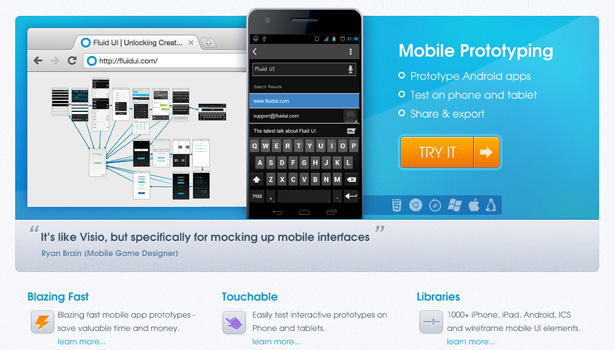
\includegraphics[scale=0.6]{fluid_ui}
			\caption[Fluid UI]{Fluid UI.}
			\label{fig:fluid_ui}
		\end{figure}

	\section[BitStrips]{\emph{BitStrips}}
	\label{sec:ferramentas_bitStrips}

		A ferramenta usada para criar o story board foi o bitstrips. Bitstrips.com é um web site onde você cria quadrinhos gratuitamente, de forma simples, mas com muitos recursos. O Bitstrips é um site sem fins lucrativos criados pela Core Matrix para criação, edição e publicação de histórias em quadrinhos, as famosas "comics", online.
		
		\newpage

		\begin{figure}[h]
			\centering
			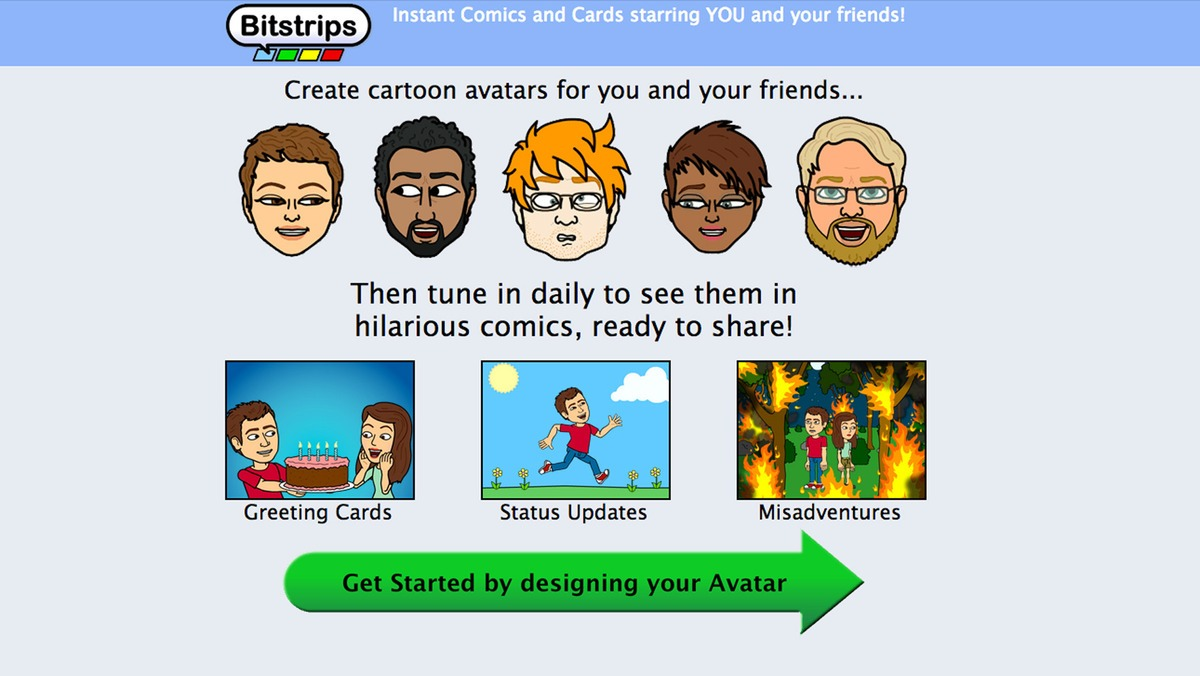
\includegraphics[scale=0.3]{bit_strips}
			\caption[BitStrips]{BitStrips.}
			\label{fig:bit_strips}
		\end{figure}